%%% The main file. It contains definitions of basic parameters and includes all other parts.

% Meta-data of your thesis (please edit)
\input metadata.tex

% Generate metadata in XMP format for use by the pdfx package
\input xmp.tex

%% Settings for single-side (simplex) printing
% Margins: left 40mm, right 25mm, top and bottom 25mm
% (but beware, LaTeX adds 1in implicitly)
\documentclass[12pt,a4paper]{report}
\setlength\textwidth{145mm}
\setlength\textheight{247mm}
\setlength\oddsidemargin{15mm}
\setlength\evensidemargin{15mm}
\setlength\topmargin{0mm}
\setlength\headsep{0mm}
\setlength\headheight{0mm}
% \openright makes the following text appear on a right-hand page
\let\openright=\clearpage

%% Settings for two-sided (duplex) printing
% \documentclass[12pt,a4paper,twoside,openright]{report}
% \setlength\textwidth{145mm}
% \setlength\textheight{247mm}
% \setlength\oddsidemargin{14.2mm}
% \setlength\evensidemargin{0mm}
% \setlength\topmargin{0mm}
% \setlength\headsep{0mm}
% \setlength\headheight{0mm}
% \let\openright=\cleardoublepage

%% If the thesis has no printed version, symmetric margins look better
% \documentclass[12pt,a4paper]{report}
% \setlength\textwidth{145mm}
% \setlength\textheight{247mm}
% \setlength\oddsidemargin{10mm}
% \setlength\evensidemargin{10mm}
% \setlength\topmargin{0mm}
% \setlength\headsep{0mm}
% \setlength\headheight{0mm}
% \let\openright=\clearpage

%% Generate PDF/A-2u
\usepackage[a-2u]{pdfx}

%% Prefer Latin Modern fonts
\usepackage{lmodern}
% If we are not using LuaTeX, we need to set up character encoding:
\usepackage{iftex}
\ifpdftex
\usepackage[utf8]{inputenc}
\usepackage[T1]{fontenc}
\usepackage{textcomp}
\fi

%% Further useful packages (included in most LaTeX distributions)
\usepackage{amsmath}        % extensions for typesetting of math
\usepackage{amsfonts}       % math fonts
\usepackage{amsthm}         % theorems, definitions, etc.
\usepackage{bm}             % boldface symbols (\bm)
\usepackage{booktabs}       % improved horizontal lines in tables
\usepackage{caption}        % custom captions of floating objects
\usepackage{dcolumn}        % improved alignment of table columns
\usepackage{floatrow}       % custom float environments
\usepackage{graphicx}       % embedding of pictures
\usepackage{indentfirst}    % indent the first paragraph of a chapter
\usepackage[nopatch=item]{microtype}   % micro-typographic refinement
\usepackage{paralist}       % improved enumerate and itemize
\usepackage[nottoc]{tocbibind} % makes sure that bibliography and the lists
			    % of figures/tables are included in the table
			    % of contents
\usepackage{xcolor}         % typesetting in color

% The hyperref package for clickable links in PDF and also for storing
% metadata to PDF (including the table of contents).
% Most settings are pre-set by the pdfx package.
\hypersetup{unicode}
\hypersetup{breaklinks=true}

% Packages for computer science theses
\usepackage{algpseudocode}  % part of algorithmicx package
\usepackage{algorithm}
\usepackage{fancyvrb}       % improved verbatim environment
\usepackage{listings}       % pretty-printer of source code

% You might want to use cleveref for references
% \usepackage{cleveref}

% Set up formatting of bibliography (references to literature)
% Details can be adjusted in macros.tex.
%
% BEWARE: Different fields of research and different university departments
% have their own customs regarding bibliography. Consult the bibliography
% format with your supervisor.
%
% The basic format according to the ISO 690 standard with numbered references
\usepackage[natbib,style=iso-numeric,sorting=none]{biblatex}
% ISO 690 with alphanumeric references (abbreviations of authors' names)
%\usepackage[natbib,style=iso-alphabetic]{biblatex}
% ISO 690 with references Author (year)
%\usepackage[natbib,style=iso-authoryear]{biblatex}
%
% Some fields of research prefer a simple format with numbered references
% (sorting=none tells that bibliography should be listed in citation order)
%\usepackage[natbib,style=numeric,sorting=none]{biblatex}
% Numbered references, but [1,2,3,4,5] is compressed to [1-5]
%\usepackage[natbib,style=numeric-comp,sorting=none]{biblatex}
% A simple format with alphanumeric references:
%\usepackage[natbib,style=alphabetic]{biblatex}

% Load the file with bibliography entries
\addbibresource{bibliography.bib}

% Our definitions of macros (see description inside)
\input macros.tex

%%% Title page and various mandatory informational pages
\begin{document}
\include{title}

%%% A page with automatically generated table of contents of the thesis

\tableofcontents

%%% Each chapter is kept in a separate file
\chapter*{Introduction}
\addcontentsline{toc}{chapter}{Introduction}

Data Quality Management (DQM) refers to the processes, technologies, and practices used to maintain high quality in data through its lifecycle. It encompasses the acquisition, implementation, and control of data accuracy, completeness, reliability, and relevance in enterprise systems. DQM ensures that data remains accurate, consistent, and accessible across all platforms and applications within an organization.
Importance for Modern Enterprises

In the age of big data and advanced analytics, data quality management is not just a luxury—it's an imperative. DQM is critical for modern enterprises for many reasons, including the following:

\begin{itemize}
    \item   Informed Decision-Making
    
    High-quality data is pivotal for accuracy in decision-making. Decisions based on inaccurate or incomplete data can lead to significant financial losses and strategic missteps.

    \item   Regulatory Compliance
    
    Many industries are subject to regulations that mandate the integrity and confidentiality of data. For example, the GDPR in Europe and HIPAA in the United States impose strict guidelines on data privacy and the quality of information that is stored and processed.
        DQM helps organizations comply with these regulations and avoid hefty penalties by ensuring data is managed correctly throughout its lifecycle.

    \item   Enhanced Customer Satisfaction

    Data quality directly impacts customer experience. Accurate customer data helps businesses understand their clients better, tailor their interactions more effectively, leading to improved customer satisfaction and loyalty.

    \item Operational Efficiency
    
    High-quality data reduces errors and the need for rework. For instance, accurate inventory data helps in managing stock levels efficiently, avoiding overstocking or stockouts.
    By automating data cleansing and enrichment, organizations can streamline workflows and allow employees to focus on higher-value activities rather than correcting data errors.    

    \item     Risk Mitigation

    Poor data quality is a major risk in itself—it can skew analysis, leading to misguided strategies that may harm the business.
    DQM practices identify and correct discrepancies in data before they propagate through the enterprise, thereby mitigating risks associated with data handling and storage.

\end{itemize}





\chapter{Analysis}
As we established in introduction, there are many benefits to having DQM processes in place. In fact, in today's data-driven environments, the assurance of data quality is not just a preference but a critical necessity. Organizations rely on accurate, timely, and reliable data to make informed decisions, drive strategies, and optimize operations. As such, the field of data quality management has evolved to address these needs through sophisticated tools and methodologies. However, the effective implementation of these tools requires a deep understanding of both the tools themselves and the roles of those who interact with them.


This chapter delves into the analysis of the current landscape of data quality management, focusing particularly on the need for programmatic access to these tools. This need stems from the growing requirement to seamlessly integrate data quality solutions into existing data pipelines, a task that typically falls within the purview of data engineers. As we explore this topic, we will discuss the challenges faced by data engineers and the crucial role of data stewards in ensuring the success of data quality initiatives. The insights gained here will lay the groundwork for understanding how programmatic access can bridge the gap between manual data quality oversight and automated, scalable data governance frameworks.


\section{The need for programmatic access}

In context of data quality management, most commonly the centerpoint of the focus is on the personal of the so called 'data steward'. The reason for this is that data stewards are crucial
for any kind of data quality initiative. Data stewards need to be involved with the setup of data quality process to ensure its success. This includes many tasks such as defining data quality rules,
data profiling, and addressing data quality issues. [What is a data steward? https://www.ataccama.com/blog/what-is-a-data-steward]

In the world of data quality management, there arises a need to consume data quality tools programatically. This is where the persona of a data engineer comes into play. There are more reasons for this, in simple terms,
the necessity is a collaraly to the need to integrate data quality tools into data pipelines. Enter the data engineer. Data engineers are responsible for the development of data pipelines, and the integration of data quality tools into these pipelines. 

The need for programmatic access to data quality tools is dictated by the need to integrate data quality tools into data pipelines. Data engineers are responsible for the development of data pipelines, and the integration of data quality tools into these pipelines. It follows that any solution aimed at pipeline integration and so at data engineers should be designed to accommodate for this. In the following sections, we will discuss the needs of data engineers in the context of data quality management tools.

\section{Data Quality Management Tools at Ataccama}

One of the major players in the field of dq management tools is Ataccama. 

Ataccama ONE is a data management application that provides a wide range of features for data quality management, such as Data cataloging, Master data management, and Data visualisations. Most importantly, Ataccama ONE includes a wide suite of data quality management tools. This includes data profiling, data quality rules, data quality monitoring, and data quality issue resolution. Ataccama ONE also provides a wide range of connectors to various data sources and data targets.

Ataccama is a powerful tool for data quality management, but it has some limitations. One of the limitations of Ataccama ONE is that it is not designed for programmatic access. The main interface for Ataccama ONE is a web interface. This means that it is not easy to integrate Ataccama into data pipelines.

\subsection{Data Quality Rules at Ataccama}

Data quality rules are essential components of any comprehensive data management strategy, and Ataccama ONE excels in providing robust capabilities for defining and enforcing these rules. Ataccama's approach to data quality rules allows businesses to ensure that their data conforms to specific standards and requirements, crucial for accurate, reliable, and actionable data insights.

Data quality rules in Ataccama are closely integrated with the platform's data governance capabilities. This integration ensures that the enforcement of data quality is aligned with broader data governance frameworks and compliance requirements. Rules can be linked to specific data governance policies, providing traceability and accountability.

Ataccama ONE's data quality management features are both robust and comprehensive, making it an exemplary foundation for any organization's data quality initiatives. The platform's extensive capabilities in defining, applying, monitoring, and resolving data quality issues position it as an ideal choice for those looking to enforce stringent data quality standards. With its rich suite of tools for data profiling, quality rule creation, and issue management, Ataccama ONE is well-equipped to handle the diverse and complex data landscapes of modern enterprises. Given its strong feature set and integration potential, we will base our solution on Ataccama's proven frameworks to ensure that our data governance and quality management efforts are both effective and efficient.

\section{The persona of Data engineer and their needs}

As we have established earlier, data engineers are the key persona for the integration of data quality tools into data pipelines. It is good practice to tailor application to the its users and their requirements. It follows that any solution aimed at pipeline integration should take into account the needs of data engineers.

Data engineers like any others are working professionals. Many of them are used to working with some particular tools and technologies. It is important to take into account the tools and technologies that data engineers are familiar with when designing a solution for them.

Although between many data engineers there are differences in the tools and technologies they use, there are some common tools and technologies that are used by the majority of them in today's world. It is important to realize that we should not only consider an ideal data engineer, a skilled senior, but also take into account that there are many junior data engineers. Also, it is important to consider the cognitive load of new tools and technologies on data engineers. Not only need to be the tools and technologies easy to learn and use, also they should be based on familiar concepts and technologies. This way, the data engineers can focus on their work, and not on learning new tools and technologies. 

[Source needed] The most commonly used tools and technologies by data engineers are Python, Java, Scala, and SQL. These tools and technologies are used for the development of data pipelines, and the integration of data quality tools into these pipelines. For any set of data engineers, the intersection of their knowledge bases will include Python more often than anything else.

\section{Data pipelines and requirements for the integration of data quality tools}

Data pipelines are a crucial part of any data engineering project. Data pipelines are used to move data from one place to another, and to transform data from one format to another. Data pipelines are used to integrate data quality tools into data pipelines. Data engineers are responsible for the development of data pipelines, and the integration of data quality tools into these pipelines.

Many of usecases for integrating data quality tools into data pipelines include the requirement to integrate with existing data pipeline or solution. This means that the data quality tools should be able to integrate with commonly used data pipelines. It also follows that to force the use of a new data pipeline or ETL solution is a non-functional requirement. 

For example in Ataccama, the application is intended to be connected to all the data sources and data targets using its custom connectors. To access the Ataccama engine and run any sort of evaluation of data quality rules, the data either need to be loaded into Ataccama ONE using a connection setup within the application, or the data needs to be sent into a service set up from within the application. Both of these approaches present a challenge for the integration of Ataccama into existing data pipelines.

\subsection{Data security}

One of the main concerns of any data owner is data security. Sending data over the internet to a third-party service can be a security risk. This is especially true for sensitive data. Data security is a major concern for data engineers, and it is important to take into account the security requirements of data engineers when designing a solution for them.

When a data quality integration in a pipeline needs to accesa a server, an application running somewhere else, it means network access. This can be a security risk. In case of a private network, the application needs to be exposed to the network, which can introduce entirely new vectors of attack

\subsection{Ease of configuration}

The need to access a running instance of an application in order to run data quality tooling comes with added complexities.

First, the application needs to be configured and running. This is fine for an environmnent where such an application is already in use, yet still it is an added complexity as part of the process is running somewhere else and so it can be more difficult to debug, monitor, and maintain.

Second, the pipeline needs to access the application over a network. This means that the application needs to be exposed to the network, which can not only be a security risk, but also provide further complexities in terms of network configuration. In case of a private network, the application needs to be exposed to the network, which can in some cases be even out of question and make the integration impossible.

\subsection{Pipelines in commonly used data platforms}

Modern data ecosystems are diverse, with organizations leveraging a variety of data storage solutions and computing environments to manage and analyze data. Here’s how Python integration plays a critical role across commonly used platforms:

\begin{itemize}
\item  Snowflake

Snowflake supports multiple programming languages, including Java and .NET, but Python remains a popular choice due to its extensive library support and community.

Python is well-supported in Snowflake through connectors like Snowflake Connector for Python, which allows executing SQL statements and performing data manipulations directly from Python scripts.


\item AWS Glue

    AWS Glue supports Python and Scala. Python, being one of the main languages supported by AWS Glue, benefits from seamless integration with other AWS services.
    
    Python scripts in AWS Glue can perform extract, transform, and load (ETL) tasks effectively, which can be developed and debugged directly in Python using Glue’s development endpoints.


    \item Azure Data Factories

    Azure Data Factory (ADF) supports custom activities in various languages, but Python’s use in Azure functions for custom processing activities is notable due to its simplicity and effectiveness.
   
    Python in ADF can be used to orchestrate complex data workflows, invoking Python-based processes as part of the data integration pipelines.


    \item Databricks

    Databricks offers a unified analytics platform that supports Python, Scala, SQL, and R. Python’s integration, particularly with PySpark for big data processing, makes it a primary choice for many developers.

    Python is extensively used in Databricks notebooks for data exploration, visualization, and machine learning, highlighting its versatility and ease of use.

\end{itemize}


Given the need to operate within commonly used compute platforms such as the above mentioned, it is imperative to consider the compatibility of programming languages supported by these environments. Each platform offers support for various technologies; however, Python stands out due to its universal acceptance and extensive integration capabilities across these systems. Whether it is executing complex data manipulation tasks in Snowflake, orchestrating ETL processes in AWS Glue, running custom activities in Azure Data Factory, or performing data analysis and machine learning in Databricks, Python is consistently supported. Therefore, focusing on Python for implementing data quality rules not only aligns with the operational capabilities of these platforms but also ensures that our solutions are versatile and adaptable across different technological ecosystems. This strategic choice maximizes the utility and reach of our data quality management tools, making them accessible and functional within the predominant data processing frameworks employed by contemporary organizations.

\section{Similar Solutions}

This section compares Ataccama ONE to other data quality management tools that are designed for programmatic access, highlighting the relative strengths and limitations of each solution in terms of features, technology stack, and integration capabilities.

\subsection{Soda Core}

Soda Core is a robust open-source tool tailored for integrating data quality checks directly into data pipelines. However, its feature set primarily focuses on:

\begin{itemize}
    \item Data Monitoring and Alerting
    
    Automatically detecting and alerting on anomalies in data as it flows through pipelines.

    \item Customizable Quality Checks

    While flexible, these are generally more basic compared to the depth provided by comprehensive DQM platforms.

    \item Python Integration
    
    Strong integration with Python-based data ecosystems, suitable for teams relying heavily on Python for data processing.
\end{itemize}

\subsection{Great Expectations}

Great Expectations offers a framework for setting up complex data validation and documentation, which is crucial for maintaining high data quality standards. Its key features include:

\begin{itemize}
    \item   Validation Framework
    
    Extensive support for defining expectations about data, which can be automatically validated against data batches.

    \item Data Docs
    
    Automatically generated documentation that helps keep teams aligned on data quality standards.

    \item Integration
    
    While it offers broad integration capabilities, it requires significant setup and maintenance compared to more out-of-the-box solutions.
\end{itemize}


\subsection{Comparison with Ataccama ONE}

Ataccama ONE offers a more extensive suite of features than either Soda Core or Great Expectations. This includes advanced functionalities like Master Data Management, Data Cataloging, and enriched Metadata Management, which are not typically found in the aforementioned open-source tools.

Ataccama integrates machine learning and AI-driven insights into its platform, providing a more sophisticated analysis and automation level than Soda Core and Great Expectations typically offer.

Despite its robust feature set, Ataccama’s main limitation lies in its less flexible integration with Python-based data pipelines, which is where Soda Core and Great Expectations excel due to their native Python support.

\section{Enhancing Ataccama's Integration Capabilities}

Given the comprehensive features of Ataccama ONE, the focus of this thesis will shift towards enhancing its integration capabilities with Python-based data pipelines to leverage its extensive data quality functionalities more effectively in programmatic environments.

While Ataccama offers a superior range of features, enhancing its programmatic accessibility would significantly increase its utility in modern data environments. This thesis will explore feasible solutions to bridge this gap, thereby extending the powerful capabilities of Ataccama ONE to a broader range of applications and use cases.


\chapter{Design}

The design section of this thesis serves as a bridge between the theoretical analysis and the practical implementation of the project. This section should comprehensively outline the proposed solution, coming from the goals summarized in analysis, describing design principles, methodologies, and tools to be employed. 

\section{Goals}

First step of the design process is to summarize the goals of the project. The goals of the project are derived from the analysis section of the thesis. In subsequent subsections, the goals will serve as a base for making design decisions. 


\subsection{Compatibility with the Ataccama Expression Language}

In Ataccama, data quality rules are defined using a custom expression language Ataccama Expressions. 

The solution should be designed to be compatible with Ataccama Expressions, most importantly, a user should be able to reuse data quality rules originally written in Ataccama Expression Language, and run evaluate them.

This language is defined using a formal grammar. The expected functions and operators output is defined in a separate documentation.

The goal of this project is to bring the Ataccama expression language over to Python, so that it can be executed with as little managed dependecies as possible. This means that the language will have to be implemented in such a way that it can be executed in a Python environment without any additional dependencies except for Python packages, which are easily managable and an industry standard.


\subsection{Design an API that is easy to use for data engineers}

In the analysis section, the persona of data engineer was introduced as the main user of the solution. The main goal of the project is to design an API that is easy to use for data engineers. The API should be based on familiar concepts and technologies, and should be easy to learn and use. The API should be designed to accommodate for the needs of data engineers, and should be tailored to their requirements.

\subsection{Reasonable performance}

The API should be designed to be fast and efficient. The API should be designed to be compatible with commonly used data pipelines, and should be designed to be easy to integrate into data pipelines. The API should be designed to be secure, and should be designed to be easy to configure, debug, monitor, and maintain.

\section{Architecture}

One of the first decisions that have to be made is the architecture of the solution.

The program itself will do the following:

\begin{enumerate}
    \item Parse the input expression
    \item Evaluate the expression on a record and return the result
\end{enumerate}

In the first step, the expression will be parsed into an abstract syntaxt tree (AST). Given the complexity of the expression language, a best-fit solution will be to use a parser generator. The parser generator will take the grammar of the language as input and generate a parser that can parse the input expression, providing a way to add custom logic into the subsequent semantic analysis of the expression.

In the semantic analysis, the AST will be traversed and built into some for of executable code so that it can be evaluated on a record. The evaluation will be done in a Python environment, and the result will be returned to the user.

In the last step, the generated code will be executed on records, and the results will be returned.

\subsection{Parser generator}

For the parser generator, a specific approach is indicated. The Ataccama Expression Language implementation uses a parser generator called ANTLR. ANTLR (ANother Tool for Language Recognition) is a powerful parser generator for reading, processing, executing, or translating structured text or binary files. It's widely used to build languages, tools, and frameworks. From a grammar, ANTLR generates a parser that can build and walk parse trees. [https://www.antlr.org/] As the grammar of the Ataccama Expression Language is already defined, it is simple and robust to use adapt and reuse the grammar by also using ANTLR to generate the parser.

\subsection{Code generation}

Having decided on the parser generator, the next step is to decide how to generate the code for the expression. There are two obvious approaches at hand: Represent the expression in an object tree with execution being a recursive descent through the tree. The second approach is to generate Python code directly. This can be done using Python standard module ast, which can be used build an abstract syntax tree of the expression, and then compile it into a Python function. Alternatively, the code can be generated as a string and then executed using Python's exec function, but this approach is less safe, more error-prone, harder to debug and introduces more overhead as it adds an additional step of parsing the code.

The second approach is more efficient, as it avoids the overhead of traversing the AST, but it is also more complex, as it requires generating Python code. The first approach might appear simpler, but it is less efficient, as it requires traversing the AST and does not include the option to use compilation to Python bytecode.

Using Python as the runtime also comes with the benefit of being able to use Python's scope resolution and name hiding to implement the scoping rules of the Ataccama Expression Language, so a reimplementation can be avoided.

For these reasons, the second approach is chosen. The code will be generated as Python code using the ast module, and then compiled into a Python module.

\section{Compatibility with the Ataccama Expression language}


The goal of this project is to bring the Ataccama expression language over to
Python. However, the language is complex and has many features, along with
platform specific quirks a peculiarities. For this reason, the implementation will
not be a one-to-one copy of the language, but rather a subset of the language
features that are most commonly used with some differences in behaviour.
The differences between the Ataccama Expression Language and the Python
implementation will be outlined in detail i the following sections. As the goal
is to make the implementation as close to the original language as possible, the
differences will be kept to a minimum. Consequently, the implementation will be
able to run most of the data quality rules written in the Ataccama Expression
Language.
The rest of this section describes a high level overview of the differences that
will have to be introduced along with the reasons behind them. Most of the
differences are a result of a different underlying technology, decisions have to be
made on where to draw the line between mimicking the original language and

This section has two purposes: The first is to describe the language and its features, the second is to outline and discuss design decisions related to the individual fetatures and functionality that have to be made in order to implement the language in Python 
introducing accepting differences for the sake of simplicity and performance.

\subsection{Dynamic typing}

The Ataccama Expression Language is statically typed, following its language of implementation The Ataccama Expression Language is statically typed, following its language
of implementation which is Java. This means that the type of each variable and
expression is known at compile time compile time. This allows the compiler to
catch type errors at compile time, and to generate more efficient code. Also,
it allows for function and operator overloading, as the compiler can choose the
correct function based on the types of the arguments.
This is possible thanks to the record format being known at compile time. The
record format is a schema that defines the types of the fields in the record.
Python is dynamically typed, which means that it is possible to allow for
dynamic typing in the implementation.
On the other hand, to reimplement static typing in Python would require
aditional work like keeping track of the types of all symbols and expressions and
resolving function overloads.
Furthermore, static typing would require the user to define the record format
at compile time, which would make the API less user-friendly, which in our case
is a priority.
Considering the above stated arguments, the decision is to allow for dynamic
typing in the implementation, as it is easier to implement and more flexible.

\subsubsection{Function and operator overloading}

\subsection{Implementation scope}

The Ataccama Expression Language supports a great number of functions, in
total it is more than 150 functions.
The implementation of the language in Python will be limited to a subset of
the language features. The reasoning behind this is that many of the functions are
not commonly used, and the implementation of all of them would be a significant
effort.

The functions have been categorized by priority, and the implementation will
focus on the high and medium priority functions.
TODO add list of functions

\subsection{Arithmetic}
The Ataccama Expression Language operates, like standard types in Java, in
fixed-size bit arithmetic, i.e. 32 bits for integers and 64 bits for Python. Python,
on the other hand, uses arbitrary precision arithmetic, which means that the size
of the integers is not limited. This means that the results of arithmetic operations
can differ between the two languages.
For every day operation, the difference is not significant and it could be said
that the Python behaviour is better. However, in some use cases, the fixed-size
arithmetic is necessary, for example when working with hash tables. As the number
of these cases is limited and most of them are provided as implemented functionality,
the implementation will use Python-native arbitrary precision arithmetic and
handle fixed-size arithmetic as a special case where necessary.
Furthermore, the Ataccama Expression Language provides arithmetic operators
for division, integer division, and modulo. Python provides the same operators, but
the behaviour of the operators is different. The Ataccama Expression Language
uses integer division and modulo for integer operands, and floating-point division
and modulo for floating-point operands. Python uses integer division and modulo
for integer operands, and floating-point division and modulo for floating-point
operands. These operators will have to be implemented in a way that is compatible
with the Ataccama Expression Language.
\subsection{Null handling and null coalescing}
The way Ataccama Expression language handles nulls has a lot of aspects
which have to be addressed.
Operators handle null values in a SQL-like way, mostly returning null if any
of the operands is null. Implication for the implementation is that it will not be
possible to use native Python operators, as they do not handle null values in the
same way.
Empty strings are treated as null values, the documentation states "A null
string and an empty string are considered equal". Moreover, any empty string
returns are coalesced to null. This behaviour also has its own quirks, for example
‘1 + null == null‘ but ‘1 + "" == "1"‘, which breaks the aforementioned statement.

Furthermore, functions have to be prepared to handle null values in any of the
arguments. Most commonly, functions return null if any of the arguments is null,
so extensive null checking has to be implemented in the functions.
The implementation in Python will have to address these differences, and
provide a way to handle null values in a Python environment.
Date and floating point formatting

\section{Interface design}

There are not a lot of decision to be made in the API Design as the the public
functionality is simple: Compile expression and running.
Considering the functions of the implementation, one more area has to be
exposed to the user, and that concerns the ‘isInFile’ function, which is used to
do a lookup in a proprietary file format used by Ataccama for the purpose of
data quality rules. The ‘isInFile’ function accepts a string as its second argument
which is used as a identifier for the file. In the Ataccama environment, this is then
translated into a file which is loaded. The implementation will have to provide a
way to translate the file identifiers into files or paths so that the the lookup can
be executed in a local environment.

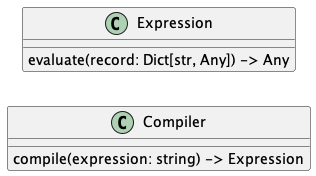
\includegraphics{diagrams/api_design-class.png}







\chapter{Design}

The design section of this thesis serves as a bridge between the theoretical analysis and the practical implementation of the project. This section should comprehensively outline the proposed solution, coming from the goals summarized in analysis, describing design principles, methodologies, and tools to be employed. 

\section{Goals}

First step of the design process is to summarize the goals of the project. The goals of the project are derived from the analysis section of the thesis. In subsequent subsections, the goals will serve as a base for making design decisions. 


\subsection{ Compatibility with the Ataccama Expression Language}

In Ataccama, data quality rules are defined using a custom expression language Ataccama Expressions. 

The solution should be designed to be compatible with Ataccama Expressions, most importantly, a user should be able to reuse data quality rules originally written in Ataccama Expression Language, and run evaluate them.

This language is defined using a formal grammar. The expected functions and operators output is defined in a separate documentation.

The goal of this project is to bring the Ataccama expression language over to Python, so that it can be executed with as little managed dependecies as possible. This means that the language will have to be implemented in such a way that it can be executed in a Python environment without any additional dependencies except for Python packages, which are easily managable and an industry standard.


\subsection{Design an API that is easy to use for data engineers}

In the analysis section, the persona of data engineer was introduced as the main user of the solution. The main goal of the project is to design an API that is easy to use for data engineers. The API should be based on familiar concepts and technologies, and should be easy to learn and use. The API should be designed to accommodate for the needs of data engineers, and should be tailored to their requirements.

\subsection{Reasonable performance}

The API should be designed to be fast and efficient. The API should be designed to be compatible with commonly used data pipelines, and should be designed to be easy to integrate into data pipelines. The API should be designed to be secure, and should be designed to be easy to configure, debug, monitor, and maintain.

\section{Architecture}

One of the first decisions that have to be made is the architecture of the solution.

The program itself will do the following:

\begin{enumerate}
    \item Parse the input expression
    \item Evaluate the expression on a record and return the result
\end{enumerate}

In the first step, the expression will be parsed into an abstract syntaxt tree (AST). Given the complexity of the expression language, a best-fit solution will be to use a parser generator. The parser generator will take the grammar of the language as input and generate a parser that can parse the input expression, providing a way to add custom logic into the subsequent semantic analysis of the expression.

In the semantic analysis, the AST will be traversed and built into some for of executable code so that it can be evaluated on a record. The evaluation will be done in a Python environment, and the result will be returned to the user.

In the last step, the generated code will be executed on records, and the results will be returned.

\subsection{Parser generator}

For the parser generator, a specific approach is indicated. The Ataccama Expression Language implementation uses a parser generator called ANTLR. ANTLR (ANother Tool for Language Recognition) is a powerful parser generator for reading, processing, executing, or translating structured text or binary files. It's widely used to build languages, tools, and frameworks. From a grammar, ANTLR generates a parser that can build and walk parse trees. [https://www.antlr.org/] As the grammar of the Ataccama Expression Language is already defined, it is simple and robust to use adapt and reuse the grammar by also using ANTLR to generate the parser.

\subsection{Code generation}

Having decided on the parser generator, the next step is to decide how to generate the code for the expression. There are two obvious approaches at hand: Represent the expression in an object tree with execution being a recursive descent through the tree. The second approach is to generate Python code directly. This can be done using Python standard module ast, which can be used build an abstract syntax tree of the expression, and then compile it into a Python function. Alternatively, the code can be generated as a string and then executed using Python's exec function, but this approach is less safe, more error-prone, harder to debug and introduces more overhead as it adds an additional step of parsing the code.

The second approach is more efficient, as it avoids the overhead of traversing the AST, but it is also more complex, as it requires generating Python code. The first approach might appear simpler, but it is less efficient, as it requires traversing the AST and does not include the option to use compilation to Python bytecode.

Using Python as the runtime also comes with the benefit of being able to use Python's scope resolution and name hiding to implement the scoping rules of the Ataccama Expression Language, so a reimplementation can be avoided.

For these reasons, the second approach is chosen. The code will be generated as Python code using the ast module, and then compiled into a Python module.

\section{Compatibility with the Ataccama Expression language}

The goal of this project is to bring the Ataccama expression language over to Python. However, the language is complex and has many features, along with platform specific quirks a peculiarities. For this reason, the implementation will not be a one-to-one copy of the language, but rather a subset of the language features that are most commonly used with some differences in behaviour.

The differences between the Ataccama Expression Language and the Python implementation will be outlined in detail i the following sections. As the goal is to make the implementation as close to the original language as possible, the differences will be kept to a minimum. Consequently, the implementation will be able to run most of the data quality rules written in the Ataccama Expression Language. 

The rest of this section describes a high level overview of the differences that will have to be introduced along with the reasons behind them. Most of the differences are a result of a different underlying technology, decisions have to be made on where to draw the line between mimicking the original language and introducing accepting differences for the sake of simplicity and performance. 

\subsection{Typing}

The Ataccama Expression Language is statically typed, following its language of implementation which is Java. This means that the type of each variable and expression is known at compile time compile time. This allows the compiler to catch type errors at compile time, and to generate more efficient code. Also, it allows for function and operator overloading, as the compiler can choose the correct function based on the types of the arguments.

This is possible thanks to the record format being known at compile time. The record format is a schema that defines the types of the fields in the record. 

Python is dynamically typed, which means that it is possible to allow for dynamic typing in the implementation. 

On the other hand, to reimplement static typing in Python would require aditional work like keeping track of the types of all symbols and expressions and resolving function overloads. 

Furthermore, static typing would require the user to define the record format at compile time, which would make the API less user-friendly, which in our case is a priority.

Considering the above stated arguments, the decision is to allow for dynamic typing in the implementation, as it is easier to implement and more flexible.

\subsection{Function overloading}

\subsection{Implementation scope}

The Ataccama Expression Language supports a great number of functions, in total it is more than 150 functions. 

The implementation of the language in Python will be limited to a subset of the language features. The reasoning behind this is that many of the functions are not commonly used, and the implementation of all of them would be a significant effort.

The functions have been categorized by priority, and the implementation will focus on the high and medium priority functions. 

TODO add list of functions

\subsection{Arithmetic}

The Ataccama Expression Language operates, like standard types in Java, in fixed-size bit arithmetic, i.e. 32 bits for integers and 64 bits for Python. Python, on the other hand, uses arbitrary precision arithmetic, which means that the size of the integers is not limited. This means that the results of arithmetic operations can differ between the two languages.

For every day operation, the difference is not significant and it could be said that the Python behaviour is better. However, in some use cases, the fixed-size arithmetic is necessary, for example when working with hash tables. As the number of these cases is limited and most of them are provided as implemented functionality, the implementation will use Python-native arbitrary precision arithmetic and handle fixed-size arithmetic as a special case where necessary.

Furthermore, the Ataccama Expression Language provides arithmetic operators for division, integer division, and modulo. Python provides the same operators, but the behaviour of the operators is different. The Ataccama Expression Language uses integer division and modulo for integer operands, and floating-point division and modulo for floating-point operands. Python uses integer division and modulo for integer operands, and floating-point division and modulo for floating-point operands. These operators will have to be implemented in a way that is compatible with the Ataccama Expression Language.

\subsubsection{Null handling and null coalescing}

The way Ataccama Expression language handles nulls has a lot of aspects which have to be addressed. 

Operators handle null values in a SQL-like way, mostly returning null if any of the operands is null. Implication for the implementation is that it will not be possible to use native Python operators, as they do not handle null values in the same way. 

Empty strings are treated as null values, the documentation states "A null string and an empty string are considered equal". Moreover, any empty string returns are coalesced to null. This behaviour also has its own quirks, for example `1 + null == null` but `1 + "" == "1"`, which breaks the aforementioned statement.

Furthermore, functions have to be prepared to handle null values in any of the arguments. Most commonly, functions return null if any of the arguments is null, so extensive null checking has to be implemented in the functions.

The implementation in Python will have to address these differences, and provide a way to handle null values in a Python environment.

\subsubsection{Date and floating point formatting}


\section{Interface design}

There are not a lot of decision to be made in the API Design as the the public functionality is simple: Compile expression and running. 

Considering the functions of the implementation, one more area has to be exposed to the user, and that concerns the `isInFile' function, which is used to do a lookup in a proprietary file format used by Ataccama for the purpose of data quality rules. The `isInFile' function accepts a string as its second argument which is used as a identifier for the file. In the Ataccama environment, this is then translated into a file which is loaded. The implementation will have to provide a way to translate the file identifiers into files or paths so that the the lookup can be executed in a local environment.


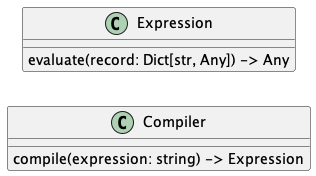
\includegraphics{diagrams/api_design-class.png}

\chapter*{Conclusion}
\addcontentsline{toc}{chapter}{Conclusion}

\xxx{The conclusion should summarize the main findings of the thesis and provide a reflection on the work done. It should also discuss the implications of the results and suggest possible directions for future research.}

%%% Bibliography
\include{bibliography}

%%% Figures used in the thesis (consider if this is needed)
\listoffigures

%%% Tables used in the thesis (consider if this is needed)
%%% In mathematical theses, it could be better to move the list of tables to the beginning of the thesis.
\listoftables

%%% Abbreviations used in the thesis, if any, including their explanation
%%% In mathematical theses, it could be better to move the list of abbreviations to the beginning of the thesis.
\chapwithtoc{List of Abbreviations}

%%% Doctoral theses must contain a list of author's publications
\ifx\ThesisType\TypePhD
\chapwithtoc{List of Publications}
\fi

%%% Attachments to the thesis, if any. Each attachment must be referred to
%%% at least once from the text of the thesis. Attachments are numbered.
%%%
%%% The printed version should preferably contain attachments, which can be
%%% read (additional tables and charts, supplementary text, examples of
%%% program output, etc.). The electronic version is more suited for attachments
%%% which will likely be used in an electronic form rather than read (program
%%% source code, data files, interactive charts, etc.). Electronic attachments
%%% should be uploaded to SIS. Allowed file formats are specified in provision
%%% of the rector no. 72/2017. Exceptions can be approved by faculty's coordinator.
\appendix
\chapter{Attachments}


\section{List of Functions}

\begin{itemize}
    \item Bitwise functions
    \begin{itemize}
        \item bitand 
        \item bitneg 
        \item bitor 
        \item bitxor 
    \end{itemize}
    \item Coding functions
    \begin{itemize}
        \item coding.md5, encode.md5 
        \item coding.fromBase64 
        \item coding.toBase64, encode.base64 
    \end{itemize}
    \item Comparison operators
    \begin{itemize}
        \item <= 
        \item <>, != 
        \item < 
        \item =, == 
        \item > 
        \item >= 
    \end{itemize}
    \item Conditional functions
    \begin{itemize}
        
\item case 
\item decode 
\item iif 
\item nvl 
    \end{itemize}
    \item Conversion functions
    \begin{itemize}
 
\item getMilliseconds 
\item math.abs 
\item math.ceil, math.ceiling 
\item math.floor 
\item math.round 
\item toFloat 
\item toInteger 
\item math.longCeil, math.longCeiling 
\item math.longFloor 
\item toLong 
\item toDate 
\item toDateTime 
\item toString 
    \end{itemize}
    \item Date functions
    \begin{itemize}
        
    \item dateAdd 
    \item dateDiff 
    \item datePart 
    \item dateTrunc 
    \item getDate 
    \item now 
    \item today 
    \item getRequestTime 
    \end{itemize}
    \item Logical operators
    \begin{itemize}
       
\item AND 
\item NOT 
\item OR 
\item XOR 
    \end{itemize}
    \item Math functions
    \begin{itemize}
  
\item math.sqrt 
\item math.acos 
\item math.asin 
\item math.atan 
\item math.cos 
\item math.e 
\item math.exp 
\item math.log 
\item math.log10 
\item math.pi 
\item math.pow 
\item math.sin 
\item math.sqr 
\item math.tan 
    \end{itemize}
    \item MinMax functions
    \begin{itemize}

        \item max 
        \item min 
        \item safeMax 
        \item safeMin 
    \end{itemize}
    \item Set operators
    \begin{itemize}
        \item is in 
        \item in 
        \item not in 
        \item is not in 
    \end{itemize}

    \item TODO rest
\end{itemize}


 is

[is not](https://www.notion.so/is-not-048f4061225140f3bcbd4142f5b98c6e?pvs=21)

[getParameterValue](https://www.notion.so/getParameterValue-4492da25bd2d4213a9f471c722df1f17?pvs=21)

[getRuntimeVersion](https://www.notion.so/getRuntimeVersion-02d29b704b9c4654a69b67392d930d18?pvs=21)

[setParameterValue](https://www.notion.so/setParameterValue-8583c79e75b847c48c02020bb284a2c8?pvs=21)

[set.contains](https://www.notion.so/set-contains-d20b2ca78c2446c199951bf72e3bc47e?pvs=21)

[set.containsExp](https://www.notion.so/set-containsExp-c6c0cdc354524c63abb3807eb93b5783?pvs=21)

[set.distinct](https://www.notion.so/set-distinct-79817147356b41ca90942c0ce097e856?pvs=21)

[set.distinctExp](https://www.notion.so/set-distinctExp-abc3a3fcb1004bc8b0c5a89f85e7ca08?pvs=21)

[set.filterExp](https://www.notion.so/set-filterExp-13fa9e8daf524374b6bbbd0d5d575131?pvs=21)

[set.indexOf](https://www.notion.so/set-indexOf-31e0238e0f8c439ab640a3d8d8a8dc84?pvs=21)

[set.indexOfExp](https://www.notion.so/set-indexOfExp-e56d0be568e14187bc5a83f1204a424f?pvs=21)

[set.item](https://www.notion.so/set-item-4a0064b788c24644921b3c62b68eb007?pvs=21)

[set.lastIndexOf](https://www.notion.so/set-lastIndexOf-9bb61ab304e14803bc6e0028c44b9660?pvs=21)

[set.lastIndexOfExp](https://www.notion.so/set-lastIndexOfExp-580473483cfb4aa3be3d12d8a9a9459b?pvs=21)

[set.mapExp](https://www.notion.so/set-mapExp-bd5ed79b71a043c69e744b7f0c7b93ba?pvs=21)

[set.size](https://www.notion.so/set-size-b28d80d9e5ff4a638373d44f2959a77f?pvs=21)

[set.sort](https://www.notion.so/set-sort-29d0175c93fa417bb352759f36d8c20e?pvs=21)

[set.subSequence](https://www.notion.so/set-subSequence-d4e25fd7eb9a4456bd76ffcc08351800?pvs=21)

[set.sumExp](https://www.notion.so/set-sumExp-d77f3b4cbade4d93a4b5d049a75dcdab?pvs=21)

[set.approxSymmetricDifference](https://www.notion.so/set-approxSymmetricDifference-2395d8d4c9134366955b19190d0c6fe2?pvs=21)

[set.difference](https://www.notion.so/set-difference-a3a5869062c24405aa17b6ffb65cd4b1?pvs=21)

[set.differenceExp](https://www.notion.so/set-differenceExp-0362b2808e094fccacd9fc8240beb526?pvs=21)

[set.differenceResult](https://www.notion.so/set-differenceResult-2be276516e734dc2932365628d0606d0?pvs=21)

[set.differenceResultExp](https://www.notion.so/set-differenceResultExp-450236ab208f4442837398f55b17bf14?pvs=21)

[set.intersection](https://www.notion.so/set-intersection-91d1a1aa8ed0474baa37b7541d9b4c89?pvs=21)

[set.intersectionExp](https://www.notion.so/set-intersectionExp-cd202abc864d433397f58a5f8b375e66?pvs=21)

[set.intersectionResult](https://www.notion.so/set-intersectionResult-d8ad2a860e1c466d8fb5349a3e66736e?pvs=21)

[set.intersectionResultExp](https://www.notion.so/set-intersectionResultExp-49a45d3f2d8c41f7be21c393071629b4?pvs=21)

[set.lcsDifference](https://www.notion.so/set-lcsDifference-461b62beb6574a58ae717bd7c993e872?pvs=21)

[set.lcsDifferenceExp](https://www.notion.so/set-lcsDifferenceExp-eb2b6cd3670041eb93f5f0ed8a6f4d21?pvs=21)

[set.lcsDifferenceResult](https://www.notion.so/set-lcsDifferenceResult-32d2fb3fbb1143968d758755df9a1cfa?pvs=21)

[set.lcsDifferenceResultExp](https://www.notion.so/set-lcsDifferenceResultExp-e03688ef4fb84441bac15553231a6070?pvs=21)

[set.lcsIntersection](https://www.notion.so/set-lcsIntersection-ef17fbd511884bd19907e8ef263aede5?pvs=21)

[set.lcsIntersectionExp](https://www.notion.so/set-lcsIntersectionExp-19c7e1e8af934b7ba0e4381533042172?pvs=21)

[set.lcsIntersectionResult](https://www.notion.so/set-lcsIntersectionResult-bde73c7ba6a4484c86746c651efe8f9c?pvs=21)

[set.lcsIntersectionResultExp](https://www.notion.so/set-lcsIntersectionResultExp-7680ccda49e0402bb539f4b1822befc2?pvs=21)

[set.lcsSymmetricDifference](https://www.notion.so/set-lcsSymmetricDifference-04b5e4304e9a41f3b735997d035969d7?pvs=21)

[set.lcsSymmetricDifferenceExp](https://www.notion.so/set-lcsSymmetricDifferenceExp-08f2af33f8b44896b21d9ccc85a3d6c9?pvs=21)

[set.lcsSymmetricDifferenceResult](https://www.notion.so/set-lcsSymmetricDifferenceResult-70c4972881b84ec7b6fa09ba5a6a62f7?pvs=21)

[set.lcsSymmetricDifferenceResultExp](https://www.notion.so/set-lcsSymmetricDifferenceResultExp-98da1b782c6e4d8397a180601134a96b?pvs=21)

[set.symmetricDifference](https://www.notion.so/set-symmetricDifference-56a223e903d74eb09e390e51e40d5e4d?pvs=21)

[set.symmetricDifferenceExp](https://www.notion.so/set-symmetricDifferenceExp-7fdf806274264091bf606156a015059c?pvs=21)

[set.symmetricDifferenceResult](https://www.notion.so/set-symmetricDifferenceResult-a9b3dafcc32142d682fcfa3865a111db?pvs=21)

[set.symmetricDifferenceResultExp](https://www.notion.so/set-symmetricDifferenceResultExp-790821c3870a4512a77171e956d0044b?pvs=21)

[set.union](https://www.notion.so/set-union-5bef326b282b40dca8bb298b910a0803?pvs=21)

[set.unionExp](https://www.notion.so/set-unionExp-387af33d46b54af6816044bdf3366782?pvs=21)

[set.unionResult](https://www.notion.so/set-unionResult-18443c8af5e14717893ce39049ef62f3?pvs=21)

[set.unionResultExp](https://www.notion.so/set-unionResultExp-e7ebeeb414ad4734b05416ab20997ec7?pvs=21)

[in](https://www.notion.so/in-5cdd8bc05ec74be7a6c860f7d9c552e5?pvs=21)

[is in](https://www.notion.so/is-in-2e45405500024a798accd3f27959941b?pvs=21)

[is not in](https://www.notion.so/is-not-in-351ef2174ca14cb294694175c16fb932?pvs=21)

[not in](https://www.notion.so/not-in-5effe74c6c3b472e83e85313b898884f?pvs=21)

[capitalize](https://www.notion.so/capitalize-65d84c769aa54104911567e1f4fb3495?pvs=21)

[containsWord](https://www.notion.so/containsWord-86feb3e0860140c6bf40dcd3f262e989?pvs=21)

[eraseSpacesInNames](https://www.notion.so/eraseSpacesInNames-2ea921c0692b4d16877a7f11e0199b7f?pvs=21)

[find](https://www.notion.so/find-ba9d506a251d49cab1cdcfbbdb51a48d?pvs=21)

[indexOf](https://www.notion.so/indexOf-351c952aba9047a49e4f7ca5207aaa0c?pvs=21)

[isInFile](https://www.notion.so/isInFile-f0a0d1aa05a24beca18803d622c82133?pvs=21)

[isNumber](https://www.notion.so/isNumber-2535ce7e2c3f45ed8e44342ee42f03a5?pvs=21)

[lastIndexOf](https://www.notion.so/lastIndexOf-0a5e61acd85f4fa9b03efee6a648cbf7?pvs=21)

[left](https://www.notion.so/left-00a1054eac0e4a2092ba42c63f3be302?pvs=21)

[length](https://www.notion.so/length-293a9d5a35074767bbd3bbfae641c8d0?pvs=21)

[lower](https://www.notion.so/lower-81024e5b1da748fa9a7acf27d089de45?pvs=21)

[matches](https://www.notion.so/matches-c2b081f144334ff2ba3e9e65134af2d6?pvs=21)

[removeAccents](https://www.notion.so/removeAccents-171af89c6dcd4386924dbb463b9f9a09?pvs=21)

[replace](https://www.notion.so/replace-51c5f3581eb944d5b9528f9f268d281c?pvs=21)

[right](https://www.notion.so/right-802ad8d9f1df4212b00e043b6bf98d3c?pvs=21)

[substituteAll](https://www.notion.so/substituteAll-568164257f2b429ab99432d7b41c508a?pvs=21)

[substr](https://www.notion.so/substr-7f036b73b5f749269b70135c4302736f?pvs=21)

[trashNonDigits](https://www.notion.so/trashNonDigits-c72549e179244e7e9bb5da24d36c3b95?pvs=21)

[trashNonLetters](https://www.notion.so/trashNonLetters-82f9bdca3eca4d9cbbb64a7d9fd23c18?pvs=21)

[trim](https://www.notion.so/trim-43c052d87e4d4a05b8a31c4bb6578120?pvs=21)

[trimLeft](https://www.notion.so/trimLeft-aea80ba235a9485783275274a9a07f6b?pvs=21)

[trimRight](https://www.notion.so/trimRight-9210818401ba4181b34b3a95f3b8db9f?pvs=21)

[upper](https://www.notion.so/upper-0c6ba9247b494e2f9f3608763ea9f1c4?pvs=21)

[word](https://www.notion.so/word-8171b4993ef841318ed8c4c43518a64b?pvs=21)

[wordCount](https://www.notion.so/wordCount-73f6f6670f6548229fda8b73bfee3017?pvs=21)

[*capitalizeWithException*](https://www.notion.so/capitalizeWithException-7c44c8e5c70846f2b0732129f2547cfd?pvs=21)

[countNonAsciiLetters](https://www.notion.so/countNonAsciiLetters-16a6c52582494d85b411caddc1e23e18?pvs=21)

[cpConvert](https://www.notion.so/cpConvert-f8ecbfe3a5ac41daa6f7fc201b2afd0e?pvs=21)

[distinct](https://www.notion.so/distinct-f33e587ca6894cc0960279be078721ad?pvs=21)

[editDistance](https://www.notion.so/editDistance-a6f8725c7ceb43b58c9d1053d03bd4a4?pvs=21)

[levenshtein](https://www.notion.so/levenshtein-14b47eed4cb84d70a6884586db8ee4b4?pvs=21)

[sortWords](https://www.notion.so/sortWords-a67385f5012b4f5e839f6dd24ecb11aa?pvs=21)

[squeezeSpaces](https://www.notion.so/squeezeSpaces-4cef11060f10450cb43f9813cbbbeeb8?pvs=21)

[substituteMany](https://www.notion.so/substituteMany-beca1dc7bcc348b1afe91820f6ec6670?pvs=21)

[hamming](https://www.notion.so/hamming-ccee8f42d2224fa4837ec30f8a7616a6?pvs=21)

[replicate](https://www.notion.so/replicate-6c654c6e11504c3da478cd4260f70478?pvs=21)

[transliterate](https://www.notion.so/transliterate-e69d2d086b6d43468336c546147e6199?pvs=21)

[trashDiacritics](https://www.notion.so/trashDiacritics-c800ebbc2a854b9c9949e20a74c3d790?pvs=21)

[diceCoefficient](https://www.notion.so/diceCoefficient-6f192fb3e4d44af7a8ca68ec7fbc2262?pvs=21)

[doubleMetaphone](https://www.notion.so/doubleMetaphone-b5a94d54ce64491ea55b8b95ff8f03a8?pvs=21)

[metaphone](https://www.notion.so/metaphone-5e3dfe3f20824b6b967a0297b687f340?pvs=21)

[ngram](https://www.notion.so/ngram-604d8fc1832d4ac9b106a86201280cce?pvs=21)

[preserveCase](https://www.notion.so/preserveCase-8ee292158af74a9dab1bd1d483b8b826?pvs=21)

[soundex](https://www.notion.so/soundex-ead42e2b2848490a93c6da158729d741?pvs=21)

[trashConsonants](https://www.notion.so/trashConsonants-d9efc81c4e654253ad4741c899c5ba8f?pvs=21)

[trashVowels](https://www.notion.so/trashVowels-87e14033aeb9436d84d3041ed3f02545?pvs=21)

[wordCombinations](https://www.notion.so/wordCombinations-4e91765ef74840728be3c8212425383e?pvs=21)

[jaccardCoefficient](https://www.notion.so/jaccardCoefficient-400591dd8fe646f0b324e2af0c1b432e?pvs=21)

[jaroWinkler](https://www.notion.so/jaroWinkler-72fd93b900b745da98e7db88f0b1c6bc?pvs=21)

\end{document}
